\chapter{Preparation for work and work order}\label{ch:preparation}

\section{Preparing the vehicle}
Follow the sequence below when replacing the factory cluster with a Digifiz dashboard:
\begin{enumerate}
    \item Remove the plastic trim covering the pedals and the lower dashboard to expose the original instrument panel.
    \item Disconnect the vehicle battery.
    \item Unplug the wiring harness from the factory instrument panel.
    \item Detach the mechanical speedometer cable, if present.
    \item Unscrew the panel from its brackets and carefully remove it from the vehicle.
    \item Route the supplied temperature and speed sensor harnesses as required.
    \item Install the Digifiz dashboard into the bracket grooves and secure it with screws.
    \item For Digifiz Replica Next, install the Volkswagen MFA sensors (or equivalents) and route their leads to the CE~1/CE~2 connectors.
    \item On \texttt{GACS}/\texttt{GARS}/\texttt{DARS}/\texttt{DACS} models, connect the labelled \texttt{MFA\_MODE}, \texttt{MFA\_RESET}, \texttt{MFA\_BLOCK}, and handbrake wires manually if the vehicle harness lacks these contacts. The second-generation Replica Next connects these signals internally by default.
    \item Plug the harnesses into the dashboard.
    \item Fit the electronic speed sensor or reconnect the mechanical cable.
    \item Reinstall the dashboard trim and pedal cover in the reverse order.
\end{enumerate}

\section{Operating the dashboard}
\begin{itemize}
    \item The dashboard powers up automatically with the ignition. The sidelights switch controls the backlight.
    \item At start-up the entire speed scale illuminates while internal diagnostics stabilise the RPM model; the display then settles on the current idle speed.
    \item Once the vehicle begins to move, the system reports the parameters listed in \Cref{ch:technical-specs}.
\end{itemize}

\subsection{MFA functions}
Six MFA pages are available:
\begin{enumerate}
    \item Daily operating time.
    \item Trip distance.
    \item Fuel consumption (not implemented on the first Replica revision).
    \item Average speed (displayed as the value multiplied by ten).
    \item Engine oil temperature (external harness required).
    \item Ambient temperature (external harness required).
\end{enumerate}
On classic Replica dashboards a capacitive touch point behind the VW badge cycles the pages; Replica Next uses an external steering-column switch. Touch durations behave as follows:
\begin{itemize}
    \item Short press (\(<1\)~s): cycle to the next MFA function.
    \item Medium press (1--3~s when no steering-column switch is fitted): switch between MFA memory blocks; the change is indicated on screen.
    \item Long press (3--7~s): reset the active MFA function (affecting consumption, trip distance, elapsed time, and average speed).
\end{itemize}

\subsection{Backlight and indicator layout}
The classic dashboard offers a manual brightness trim above the parking-light switch; Replica Next relies on automatic brightness driven by a photodiode. Manual overrides can be configured through the maintenance interfaces described in \Cref{ch:replica-setup,ch:replica-next-setup}.

The layout of the horizontal indicator block and the on-screen legend are shown in \autoref{fig:indicator-layout}.

\begin{figure}[htbp]
    \centering
    \begin{subfigure}{0.48\textwidth}
        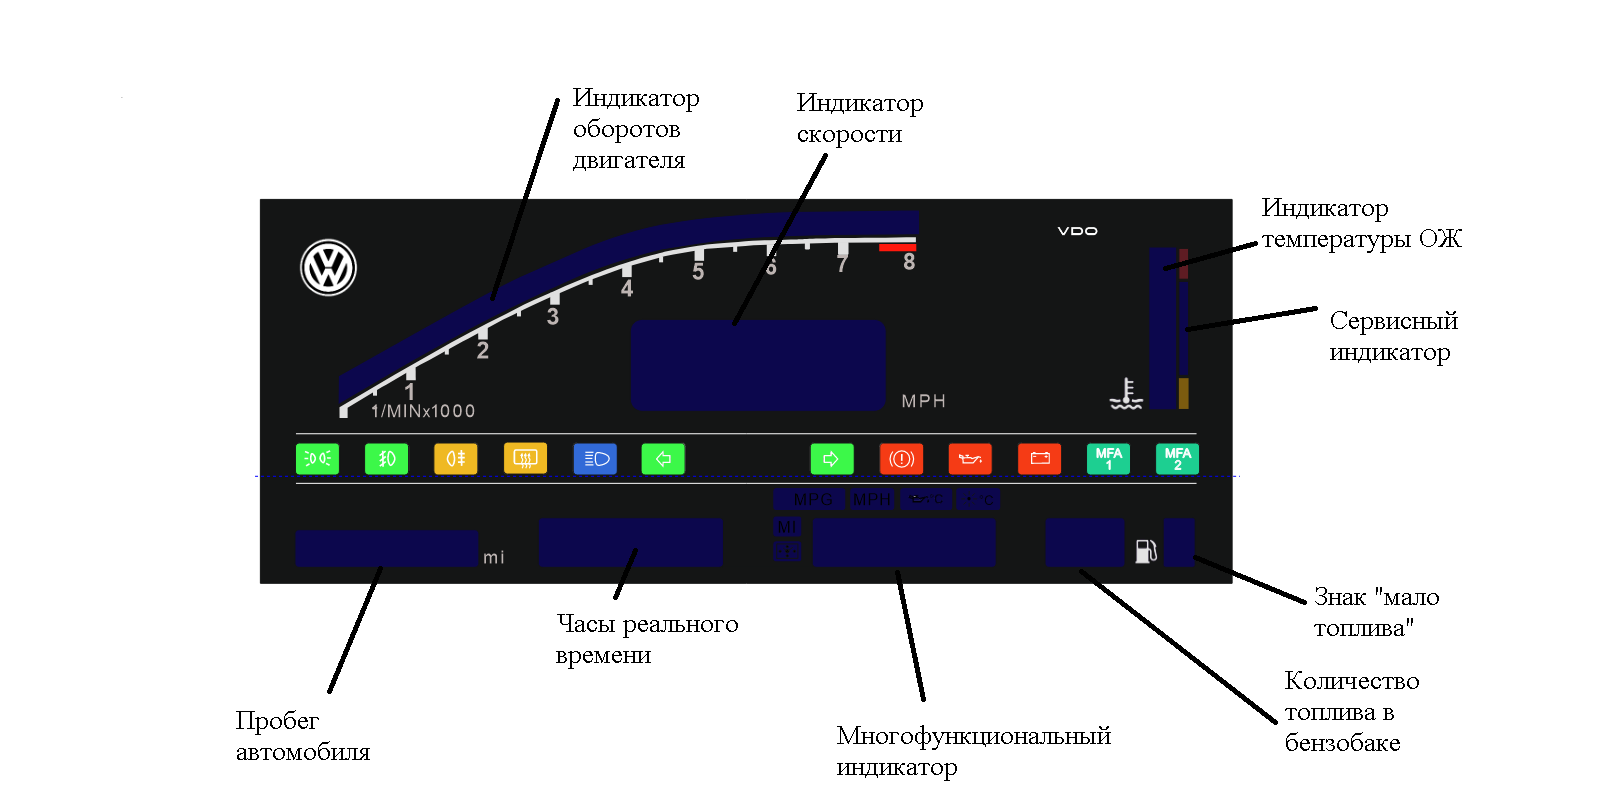
\includegraphics[width=\linewidth]{digifiz_manual/image017.png}
        \caption{Indicator layout displayed during the power-on self-test.}
    \end{subfigure}\hfill
    \begin{subfigure}{0.48\textwidth}
        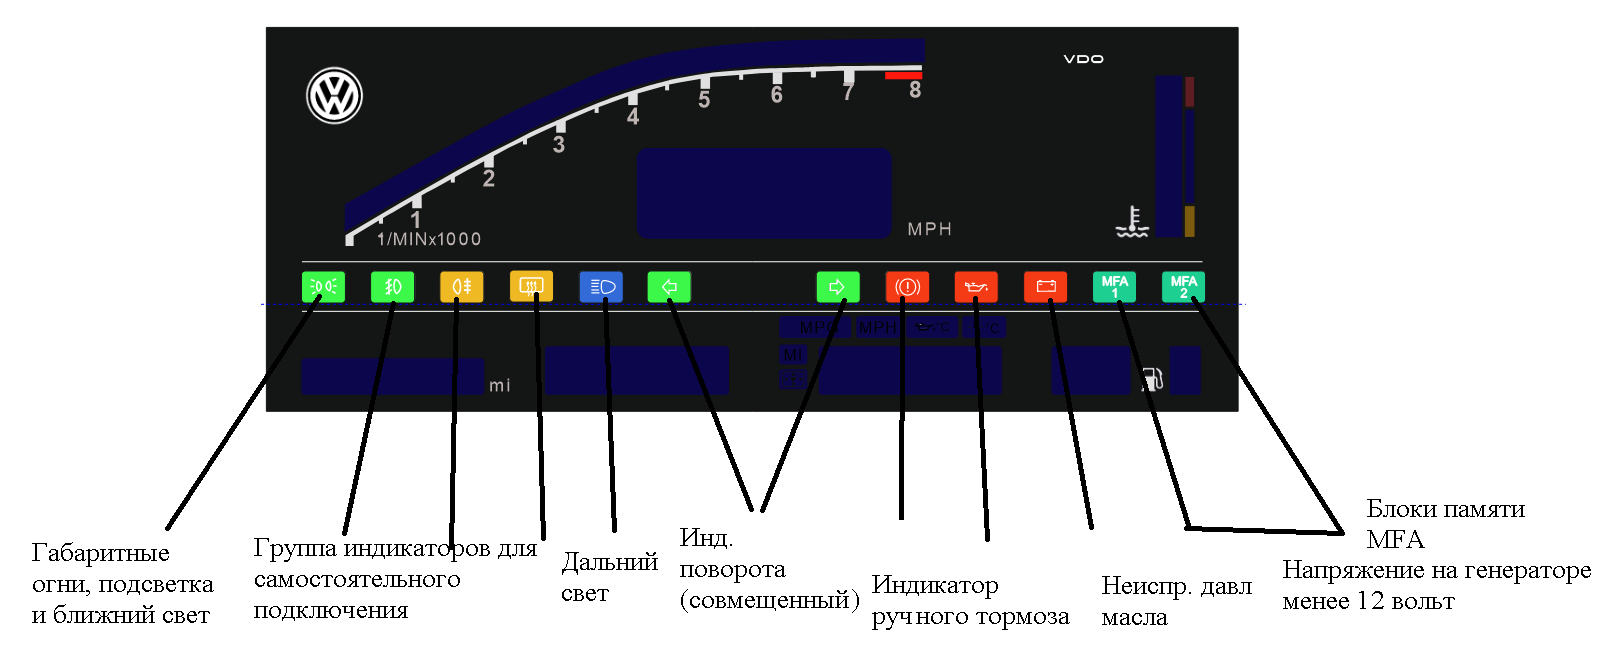
\includegraphics[width=\linewidth]{digifiz_manual/image018.png}
        \caption{Legend for the horizontal indicator group.}
    \end{subfigure}
    \caption{Instrument panel indication scheme.}
    \label{fig:indicator-layout}
\end{figure}

\subsection{Configuration interfaces}
\begin{itemize}
    \item Classic Digifiz Replica units include a Bluetooth 2.0 (or BLE-compatible) module. Install the \emph{Serial Bluetooth Terminal} application from Google Play, pair with the dashboard, and issue commands directly from the terminal view. Apple iOS devices cannot connect to this module.
    \item Replica Next exposes an embedded Wi-Fi access point and configuration portal described in \Cref{ch:replica-next-setup}. Disable mobile data while connecting to ensure the captive portal loads correctly.
\end{itemize}
Both generations can also be powered and configured on the bench using the USBasp programming interface.
